\documentclass{article}

% if you need to pass options to natbib, use, e.g.:
%     \PassOptionsToPackage{numbers, compress}{natbib}
% before loading neurips_2024


% ready for submission
% \usepackage{neurips_2024}


% to compile a preprint version, e.g., for submission to arXiv, add add the
% [preprint] option:
     \usepackage[preprint]{neurips_2024}


% to compile a camera-ready version, add the [final] option, e.g.:
%     \usepackage[final]{neurips_2024}


% to avoid loading the natbib package, add option nonatbib:
%    \usepackage[nonatbib]{neurips_2024}


\usepackage[utf8]{inputenc} % allow utf-8 input
\usepackage[T1]{fontenc}    % use 8-bit T1 fonts
\usepackage{hyperref}       % hyperlinks
\usepackage{url}            % simple URL typesetting
\usepackage{booktabs}       % professional-quality tables
\usepackage{amsfonts}       % blackboard math symbols
\usepackage{nicefrac}       % compact symbols for 1/2, etc.
\usepackage{microtype}      % microtypography
\usepackage{xcolor}         % colors
\usepackage{amsmath}
\usepackage{natbib}
\usepackage{graphicx}  % For including graphics
\usepackage{float}     % To control figure placement
\usepackage{geometry}
\usepackage{array}
\usepackage{multirow}
\usepackage{graphicx}
\usepackage{subcaption}



\title{Deep Learning 1 - Homework 2}


% The \author macro works with any number of authors. There are two commands
% used to separate the names and addresses of multiple authors: \And and \AND.
%
% Using \And between authors leaves it to LaTeX to determine where to break the
% lines. Using \AND forces a line break at that point. So, if LaTeX puts 3 of 4
% authors names on the first line, and the last on the second line, try using
% \AND instead of \And before the third author name.


\author{%
  Pedro M.P.~Curvo \\
  MSc Artificial Intelligence\\
  University of Amsterdam\\
  \texttt{pedro.pombeiro.curvo@student.uva.nl} \\
  % examples of more authors
  % \And
  % Coauthor \\
  % Affiliation \\
  % Address \\
  % \texttt{email} \\
  % \AND
  % Coauthor \\
  % Affiliation \\
  % Address \\
  % \texttt{email} \\
  % \And
  % Coauthor \\
  % Affiliation \\
  % Address \\
  % \texttt{email} \\
  % \And
  % Coauthor \\
  % Affiliation \\
  % Address \\
  % \texttt{email} \\
}


\begin{document}


\maketitle


% \begin{abstract}
%   The abstract paragraph should be indented \nicefrac{1}{2}~inch (3~picas) on
%   both the left- and right-hand margins. Use 10~point type, with a vertical
%   spacing (leading) of 11~points.  The word \textbf{Abstract} must be centered,
%   bold, and in point size 12. Two line spaces precede the abstract. The abstract
%   must be limited to one paragraph.
% \end{abstract}


\section*{Part 1}

\subsection*{Question 1.1}

\subsubsection*{a)}

The expression for $f_{1, 1}$ is given by:

\begin{equation}
    f_{1, 1} = g_{1, 1} h_{0, 0} + g_{1, 2} h_{0, -} + g_{2, 1} h_{-, 0} + g_{2, 2} h_{-, -}
\end{equation}

As we can see, we didn't use the full receptive field of the filter, since it goes beyond the image.
To address this problem, we can pad the image using several techniques, such as zero-padding, reflection padding, warp padding, etc.

\subsubsection*{b)}

\subsubsection*{b. i)}

\begin{table}[h!]
    \centering
    \resizebox{\textwidth}{!}{%
    \setlength{\tabcolsep}{4pt}
    \renewcommand{\arraystretch}{1.2}
    \begin{tabular}{|c|c|c|c|c|c|c|c|c|c|c|c|c|c|c|}
    \hline
    \multirow{2}{*}{\textbf{Type}} & \multirow{2}{*}{\textbf{Dataset}} & \multicolumn{10}{c|}{Round Accuracy (\%)} & \multirow{2}{*}{\textbf{Mean}} & \multirow{2}{*}{\textbf{Std. Dev.}} \\ \cline{3-12}
                                   &                                  &  0 &  1 &  2 &  3 &  4 &  5 &  6 &  7 &  8 &  9 &  &  \\ \hline
    \multirow{2}{*}{Valid}     & Validation & 100.0 & 100.0 & 100.0 & 100.0 & 100.0 & 100.0 & 100.0 & 100.0 & 100.0 & 100.0 & 100.0000 & 0.0000 \\ \cline{2-14}
                               & Test       & 0.3   & 0.1   & 0.0   & 0.1   & 0.0   & 0.0   & 0.1   & 0.3   & 0.0   & 0.0   & 0.0900   & 0.1136 \\ \hline
    \multirow{2}{*}{Replicate} & Validation & 98.6  & 98.1  & 98.8  & 98.5  & 97.1  & 98.8  & 98.2  & 98.0  & 98.5  & 98.5  & 98.3100  & 0.4784 \\ \cline{2-14}
                               & Test       & 92.9  & 92.8  & 88.8  & 94.7  & 95.3  & 91.7  & 96.3  & 94.7  & 95.8  & 95.0  & 93.8000  & 2.1629 \\ \hline
    \multirow{2}{*}{Reflect}   & Validation & 100.0 & 100.0 & 100.0 & 100.0 & 100.0 & 100.0 & 100.0 & 100.0 & 100.0 & 100.0 & 100.0000 & 0.0000 \\ \cline{2-14}
                               & Test       & 0.0   & 0.0   & 0.0   & 0.0   & 0.0   & 0.0   & 0.0   & 0.0   & 0.0   & 0.0   & 0.0000   & 0.0000 \\ \hline
    \multirow{2}{*}{Circular}  & Validation & 99.9  & 99.9  & 99.7  & 99.9  & 98.9  & 99.7  & 99.7  & 99.5  & 99.8  & 99.4  & 99.6400  & 0.2939 \\ \cline{2-14}
                               & Test       & 81.5  & 82.7  & 77.4  & 86.9  & 83.2  & 82.6  & 86.5  & 79.8  & 81.1  & 84.4  & 82.6100  & 2.7504 \\ \hline
    \multirow{2}{*}{sconv}     & Validation & 98.8  & 99.0  & 98.8  & 99.1  & 99.0  & 99.3  & 98.7  & 98.8  & 98.9  & 98.5  & 98.8900  & 0.2119 \\ \cline{2-14}
                               & Test       & 6.5   & 6.9   & 6.5   & 6.1   & 6.2   & 6.5   & 6.2   & 6.1   & 6.4   & 6.3   & 6.3700   & 0.2326 \\ \hline
    \multirow{2}{*}{fconv}     & Validation & 88.4  & 87.6  & 88.6  & 89.9  & 88.1  & 89.9  & 85.8  & 87.1  & 88.2  & 87.1  & 88.0700  & 1.1984 \\ \cline{2-14}
                               & Test       & 88.4  & 88.6  & 88.6  & 89.9  & 89.1  & 89.9  & 88.9  & 88.4  & 88.9  & 87.8  & 88.8500  & 0.6249 \\ \hline
    \end{tabular}
    }
    \caption{Accuracy results for Net1}
    \label{tab:results_accuracy}
\end{table}

\subsubsection*{b. ii)}
Looking at the samples from the dataset, we can observe that, for \textbf{class label 0}, a green box is on the right, and a red
box is on the left. For \textbf{class label 1}, this is reversed, with a red box on the right and a green box on the left.

While the relative positions of the green and red boxes define each class,
their absolute positions vary between the training and test sets. Looking at the README.md we observe that, in the training set,
class label 0 samples are located at the top of the image, and class label 1 samples are at the bottom. In the test set,
the positions switch: class label 0 samples are at the bottom, and class label 1 samples are at the top.
This means that the network will have to focus on learning the relative arrangement of the boxes,
which defines the class labels, rather than relying on their absolute positions in the overall image.

\subsubsection*{c)}

\subsubsection*{c i)}


The variables affecting the \texttt{conv\_type} are the \texttt{padding\_size} and the \texttt{pad\_type}.
For \textit{valid}, \textit{sconv} and \textit{fconv} we have the following differences:

\begin{itemize}
    \item \textit{valid}: No padding is added to the image, since the size of the padding is 0.
    \item \textit{sconv}: The padding added is a zero padding, with size 1.
    \item \textit{fconv}: The padding added is a zero padding, with size 2.
\end{itemize}

\textbf{Note:} Zero padding is used to add zeros to the borders of the image. The padding size determines the number of pixels added to the image in the borders.

\subsubsection*{c ii)}

If we look into the network architecture we can see that we first use a kernel size of 3 with a stride of 1 and then a stride of 2
maintaining the kernel size of 3. This configuration reduces the spatial dimensions of the feature maps during the convolution operation.

Using the \textit{valid} padding means no padding is added to the input, which results in the smallest possible output size for the convolution operation. As a result, the spatial dimensions of the feature maps are reduced, leading to less spatial information being passed to the next layer.

On the other hand, the \textit{sconv} applies a padding of 1 to the input, which slightly increases the output size of the convolution. This helps retain a bit more spatial information for the next layer.

The \textit{fconv} applies a padding of 2, which leads to a larger output size. This retains more spatial information, allowing the model to preserve more details in the feature maps as they pass to the next layer.

With that being said, we can extrapolate that larger feature maps will keep more information that allows to distinguish
between the classes in the dataset, which leads to the better performance of the model in the accuracy metric as observed. 
Hence, the order \texttt{acc\_valid} $<$ \texttt{acc\_sconv} $<$ \texttt{acc\_fconv} is expected, corresponding
to the amount of spatial information retained by the feature maps.

\subsubsection*{c iii)}

The \texttt{reflect} padding mirrors the image along its edges, while \texttt{fconv} padding uses zero padding. Reflect padding can reduce abrupt transitions at the edges by reflecting nearby pixel values. However, it can also introduce artificial patterns at the boundaries that do not exist in the original image, which may affect feature extraction and reduce the model’s ability to generalize.

In this dataset, where each image has a black background with a green and a red box, zero padding performs better. Zero-padding adds borders with zero values, which match the original black background and help the model focus on the box patterns in the center.

In contrast, \texttt{reflect} padding at all layers can create artificial features at the edges by duplicating and inverting the boxes. This can confuse the model, especially when the boxes are near the edges, as the model may confuse these artificial features created by the padding as part of the actual patterns.

\subsubsection*{c iv)}

Zero padding can dilute the information of the image by adding zero-value borders that match the original black background.
While Replicate, when the boxes are near the edges, can help maintain the boxes' patterns by extending the edge pixels into the padded area,
meaning we won't have so much dilutation of the information of the image. This makes the CNN "see" the boxes better while going
through the layers, which can lead to better performance.

Adding to this, zero padding can create a sudden change in pixel values at the image boundaries, resulting in high derivative values.
This can cause the CNN to confuse these abrupt changes with actual edges,
particularly the edges of the green and red boxes in the dataset that we are trying to predict.
In this case, this can only happen after a few layers, since the
background is black, meaning we will only have this when some information from the boxes are diffused to the edges.

Replicate padding, on the other hand, extends the edge pixels into the padded area, ensuring a smoother transition, since
the pixel will have the same value as the nearest edge pixel. This helps preserve the local context near the edges by maintaining
some statistical properties of the image, such as the derivatives. This is beneficial
when detecting the edges of the boxes. 

With these two hypothesis, we can see why the \texttt{replicate} padding performs better than the \texttt{zero} one.



\subsubsection*{d)}

\subsubsection*{d i)}
\begin{table}[h!]
    \centering
    \resizebox{\textwidth}{!}{%
    \setlength{\tabcolsep}{4pt}
    \renewcommand{\arraystretch}{1.2}
    \begin{tabular}{|c|c|c|c|c|c|c|c|c|c|c|c|c|c|c|}
    \hline
    \multirow{2}{*}{\textbf{Type}} & \multirow{2}{*}{\textbf{Dataset}} & \multicolumn{10}{c|}{Round Accuracy (\%)} & \multirow{2}{*}{\textbf{Mean}} & \multirow{2}{*}{\textbf{Std. Dev.}} \\ \cline{3-12}
                                   &                                  &  0 &  1 &  2 &  3 &  4 &  5 &  6 &  7 &  8 &  9 &  &  \\ \hline
    \multirow{2}{*}{Valid}     & Validation & 100.0 & 100.0 & 100.0 & 100.0 & 100.0 & 100.0 & 100.0 & 100.0 & 100.0 & 100.0 & 100.0000 & 0.0000 \\ \cline{2-14}
                               & Test       & 0.0   & 0.0   & 0.0   & 0.0   & 0.0   & 0.0   & 0.0   & 0.0   & 0.0   & 0.0   & 0.0000   & 0.0000 \\ \hline
    \multirow{2}{*}{Replicate} & Validation & 100.0 & 100.0 & 100.0 & 100.0 & 100.0 & 100.0 & 100.0 & 100.0 & 100.0 & 100.0 & 100.0000 & 0.0000 \\ \cline{2-14}
                               & Test       & 0.0   & 0.0   & 0.0   & 0.0   & 0.0   & 0.0   & 0.0   & 0.0   & 0.0   & 0.0   & 0.0000   & 0.0000 \\ \hline
    \multirow{2}{*}{Reflect}   & Validation & 100.0 & 100.0 & 100.0 & 100.0 & 100.0 & 100.0 & 100.0 & 100.0 & 100.0 & 100.0 & 100.0000 & 0.0000 \\ \cline{2-14}
                               & Test       & 0.0   & 0.0   & 0.0   & 0.0   & 0.0   & 0.0   & 0.0   & 0.0   & 0.0   & 0.0   & 0.0000   & 0.0000 \\ \hline
    \multirow{2}{*}{Circular}  & Validation & 100.0 & 100.0 & 100.0 & 100.0 & 100.0 & 100.0 & 100.0 & 100.0 & 100.0 & 100.0 & 100.0000 & 0.0000 \\ \cline{2-14}
                               & Test       & 0.0   & 0.0   & 0.0   & 0.0   & 0.0   & 0.0   & 0.0   & 0.0   & 0.0   & 0.0   & 0.0000   & 0.0000 \\ \hline
    \multirow{2}{*}{sconv}     & Validation & 100.0 & 100.0 & 100.0 & 100.0 & 100.0 & 100.0 & 100.0 & 100.0 & 100.0 & 100.0 & 100.0000 & 0.0000 \\ \cline{2-14}
                               & Test       & 0.0   & 0.0   & 0.0   & 0.0   & 0.0   & 0.0   & 0.0   & 0.0   & 0.0   & 0.0   & 0.0000   & 0.0000 \\ \hline
    \multirow{2}{*}{fconv}     & Validation & 100.0 & 100.0 & 100.0 & 100.0 & 100.0 & 100.0 & 100.0 & 100.0 & 100.0 & 100.0 & 100.0000 & 0.0000 \\ \cline{2-14}
                               & Test       & 0.0   & 0.0   & 0.0   & 0.0   & 0.0   & 0.0   & 0.0   & 0.0   & 0.0   & 0.0   & 0.0000   & 0.0000 \\ \hline
    \end{tabular}
    }
    \caption{Accuracy results for Net2}
    \label{tab:results_accuracy_net2}
\end{table}

\subsubsection*{d ii)}

As we can observe by the results, the model, in \texttt{Net2}, is able to achieve 100\% accuracy on the validation set for all padding types, 
but it fails to generalize to the test set, achieving 0\% accuracy, performing worse in every padding type
with lower accuracies compared to \texttt{Net1}. Since we are getting 100\% accuracy in the validation set and 0\% accuracy in the test set,
we might suspect of overfitting. 

\subsubsection*{d iii)}

In the implementation of \texttt{Net2}, an additional linear layer was added, and the AdaptiveMaxPool2d layer was removed.
The inclusion of this extra linear layer significantly increases the number of parameters in the model, which can lead to overfitting.

If we look into the \texttt{utils.py} file, we can see the the test dataset is shifted by 16 pixels relative to the validation
and training dataset. By taking this into account, we might speculate that the model \texttt{Net2} may be overfitting to the training and validation dataset
by memorizing the overall positions of the boxes in the image and, since they are shifted in the test dataset, the model is unable to
generalize to the test dataset, leading to the 0\% accuracy. That is, the model can only work on the specific positions of the boxes
in the training and validation dataset, but not in other positions of the image.

This interpretation is also supported by the observation that Net2 achieves 100\% accuracy on the validation set while
consistently scoring 0\% on the test set, regardless of the padding type.

\subsection*{Question 1.2}

\subsubsection*{a)}

% Include image the plot of inference respect to angle of rotation 
\begin{figure}[H]
    \centering
    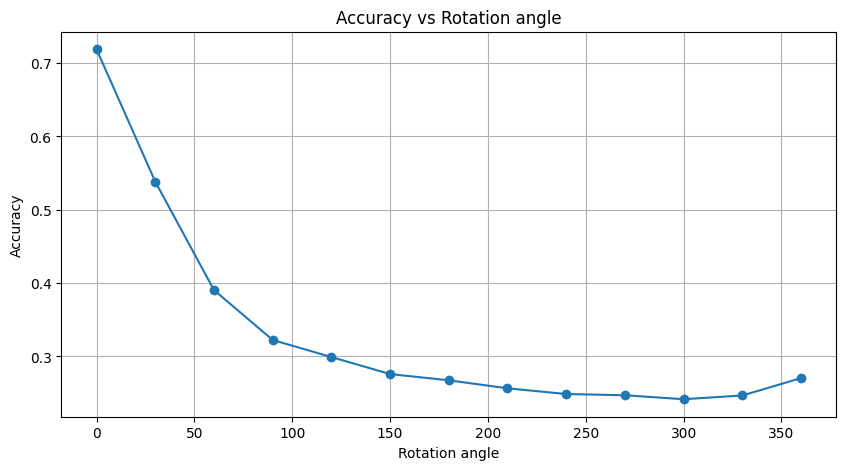
\includegraphics[width=0.8\textwidth]{images/rot_angles.png}
    \caption{Inference respect to angle of rotation}
    \label{fig:angle_inference}
\end{figure}

As we can see by the graph above, the model's accuracy decreases as the angle of rotation deviates from 0°
and exhibits symmetry around 180°. The model performs relatively better at specific angles, such as 90°, 180°, and 270°,
compared to neighboring angles. This behavior occurs because the model was trained on images with a fixed orientation,
and the filters it learned are sensitive to the orientation of features.

CNNs are not inherently rotationally invariant. The filters they learn during training are designed to detect patterns,
such as edges and textures, in specific directions. When images are rotated, the spatial alignment between these filters
and the features changes, causing a drop in accuracy. Rotating an image alters the spatial relationships between features,
making it harder for the network to recognize patterns. That is why the model performs drops in accuracy when the images are rotated.

Without training on rotated images, the model cannot generalize to recognize objects or patterns from different angles.
This limitation causes the CNN to be dependent on the orientation of the test images. One way to address this issue is to
augment the training data with rotated versions of the images. By exposing the model to a variety of orientations during training,
it can learn to detect features regardless of the angle, leading to improved performance on rotated images during inference.

\subsubsection*{b)}

% Include image the plot of inference respect to angle of rotation
\begin{figure}[H]
    \centering
    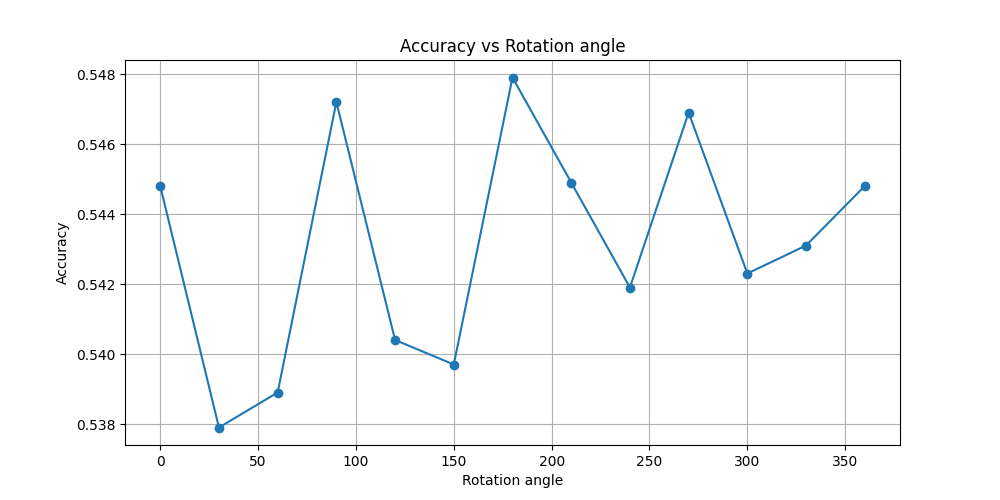
\includegraphics[width=0.8\textwidth]{images/rot_angles_aug.png}
    \caption{Inference respect to angle of rotation with data augmentation}
    \label{fig:angle_inference_aug}
\end{figure}

As seen in the graph above, the model's accuracy is more stable across different angles of rotation when trained on an augmented dataset, although
the accuracy for the unrotated images is slightly lower than the model trained on the non-augmented dataset. Again, we also observe
spikes in accuracy at specific angles, such as 90°, 180°, and 270°.

When the model is trained on an augmented dataset with random rotations, it is exposed to a variety of orientations for
the objects in the images. This allows the model to learn features that are not dependent on a specific orientation. By
using rotated versions of the images during training, the model learns to recognize patterns and objects regardless
of their angle. This helps the network develop rotational invariance, as the filters it learns become capable of detecting
the same features from different perspectives.

As a result, the model becomes more robust to rotation, and its accuracy stabilizes across different angles.
With this approach, the network does not rely on a fixed alignment of the features, and can generalize across
to more orientations. This is, again, showed by the graph above.

\newpage

\section*{Part 2}

\subsection*{Question 2.1}

\subsubsection*{a)}

\begin{itemize}
    \item Long input sequences can be challenging for Transformers due to the quadratic complexity of the self-attention mechanism, 
    that is, in self-attention, each token attends to every other token in the sequence, hence we have a  
    $O(n^2)$ complexity. This can lead to both memory
    and computational issues, which are worse when $n$ is large (larger sentences), creating bottlenecks.

    \item One way to solve this problem is by using some kind of sparse attention mechanism that focus on a subset
of local or key tokens, instead of a global attention. With this we can reduce the complexity of the self-attention mechanism. For example,
the Reformer model \textbf{(Kitaev, N., Kaiser, Ł., \& Levskaya, A. (2020). Reformer: The Efficient Transformer)}
uses locality-sensitive hashing to achieve a $O(n \log n)$ complexity.
\end{itemize}

\subsubsection*{b)}

CNNs have a local receptive field that allows them to capture local patterns in the input data and which is done
by the convolution operation between the input and a kernel filter. The initial layers in a CNN capture local, low-level
features and deeper layers combines them progressively, meaning the receptive field increases with network depth. This means
that a exponential growth is required to capture long-range dependencies in the input data, which can be a limitation
for CNNs in some tasks.

One the other hand, Transformers have a global
receptive field that allows them to capture long-range dependencies in the input data, which is done by the self-attention
mechanism, since it allows each token to attend to every other token in the sequence. That is, we have an immediate
global context in a single layer at a computational cost of $O(n^2)$, which, however, can be a limitation for long input sequences.

\subsubsection*{c)}

The scaling factor $\frac{1}{\sqrt{d_k}}$ is used to stabilize the gradients during training. The dot product of the
$Q$ and $K$ matrices is scaled by $\frac{1}{\sqrt{d_k}}$ to prevent the dot products from becoming too large when the
dimensionality of the keys $d_k$ is high. If it were the case that some values were too large, the softmax function would
produce gradients that are too small, leading to slower learning or vanishing gradients which would harm the gradient descent process.

The choice for $d_k$ arises from the variance of the dot product of two random vectors. If we have two random vectors $x$ and $y$
with zero mean and unit variance, the variance of their dot product is $d_k$. By scaling the dot product by $\frac{1}{\sqrt{d_k}}$,
we ensure that the variance of the dot product is 1, which helps stabilize the gradients during training.
(https://github.com/BAI-Yeqi/Statistical-Properties-of-Dot-Product/blob/master/proof.pdf)

\subsubsection*{d)}

If we assume we have the same total computation cost, then the multiple attentions heads are beneficial because they allow
to capture different types of dependencies and patterns simultaneously.
With a single head we can only learn a single representation and we are forced to attend to all tokens with the same
learned weights, meaning we have a limited ability to capture different patterns in the input sequence.
With multihead attention, each head learns a different representation subspace, meaning we can have different patterns
captured by different heads that are extracting it in parallel. 

This can also help mitigate some bias that can originate in some
heads due to the dominance of some tokens and can help improve generalization because, by learning multiple sets of
attention parameters, the model can be more robust to different tasks.

\subsection*{Question 2.2}

\textcolor{blue}{CODE}

\subsection*{Question 2.3}

\subsubsection*{a to b)}
\textcolor{blue}{CODE}

\subsubsection*{c)}

The MLP head is wide and not deep for several factors.
\begin{itemize}
    \item We want to keep a degree of independence of tokens in the MLP, meaning we don't need a deep network to capture
    long dependencies between the tokens. With a wide network, we are basically representing each token in a higher-dimensional
    space, which can help to capture more complex patterns independently. If we employed a deep network, we would be
    capturing deeper dependencies between tokens, which is not necessary in this case, since the self-attention mechanism already
    does it.
    \item Wide networks are better for parallelization, that is, we can split the model across multiple
    GPUs, which can lead to more computational efficiency. 
    \item Fewer layers can reduce vanishing gradient problems and are easier to optimize. Hence, by keeping the MLP shallow, we also reduce the probability of overfitting
    and can keep a more stable training process.
\end{itemize}


\subsection*{Question 2.4}

\subsubsection*{a)}

If we do not use a positional embedding, the Transformer model will not be able to distinguish the order of the tokens in the
input sequence. This is because the self-attention mechanism treats all tokens as independent, and without positional information,
meaning is permutation invariant. For example, without positional embeddings, the model would treat the sentences "The dog bit the man"
and "The man bit the dog" as the same, which is not the desired behavior. We need to have a positional embedding
for a sequential structure, specially for tasks like syntax, etc... which are characteristics of language tasks that we
want the model to learn.

\subsubsection*{b)}

By using absolute position embeddings, that is, by assigning, for example, 1 to the first token, 2 to the second token, and so on,
we are restricting the model to work within the predefined sequence length. This can be problematic if we then want to apply the model
to sequences that are longer than the ones seen during training. Besides that, we can have, for example, different types of inputs, 
where lengths can vary, for example, documents, translation tasks, etc... In these cases, the model would not be able to generalize.
Adding to this, we also want the model to have a sense of proximity between tokens, which is not achieved by absolute position embeddings.
For example, we might want the model to understand that the tokes "The" and "dog" appear closer than "man" and "dog".

By using relative position embeddings, we can overcome these limitations. Relative position embeddings allow the model to learn
the relative distances between tokens, which can be more useful in tasks where the absolute position of tokens is not as important.
Adding to this, the model can then extrapolate to different new sequences lengths and can even retain the context in large
sequences, for example, in resuming tasks, where we have large documents.


\subsection*{Question 2.5}

\textcolor{blue}{CODE}

\subsection*{Question 2.6}

\textcolor{blue}{CODE}

\subsection*{Question 2.7}

% Insert image with epochs
\begin{figure}[H]
    \centering
    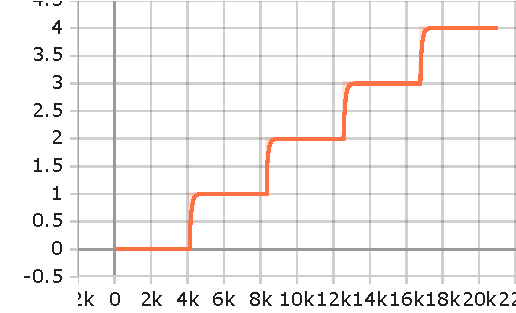
\includegraphics[width=0.8\textwidth]{images/epoch.pdf}
    \caption{Epochs per Step}
    \label{fig:loss_epochs}
\end{figure}

% Insert image with Train Acc Epoch 

\begin{figure}[H]
    \centering
    \begin{subfigure}{0.48\textwidth}  % Adjust the width to your preference
        \centering
        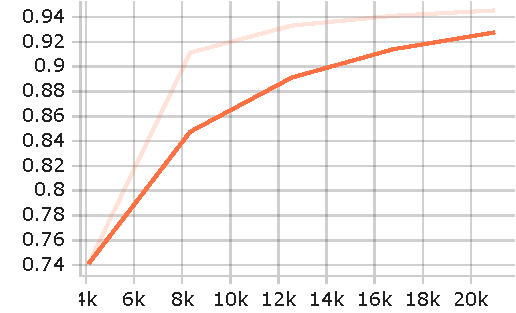
\includegraphics[width=\textwidth]{images/train_acc_epoch.pdf}
        \caption{Train Accuracy per Epoch}
        \label{fig:train_acc_epochs}
    \end{subfigure}
    \hfill
    \begin{subfigure}{0.48\textwidth}
        \centering
        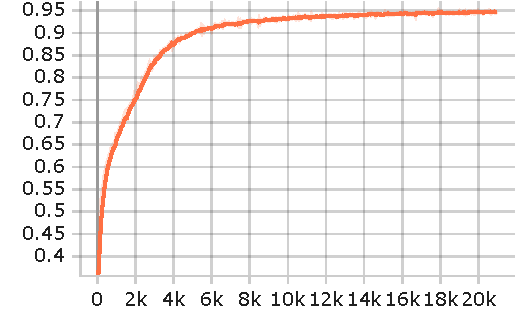
\includegraphics[width=\textwidth]{images/train_acc_step.pdf}
        \caption{Train Accuracy per Step}
        \label{fig:train_acc_steps}
    \end{subfigure}
\end{figure}

% Insert image with Train Loss per Epoch

\begin{figure}[H]
    \centering
    \begin{subfigure}{0.48\textwidth}  % Adjust the width to your preference
        \centering
        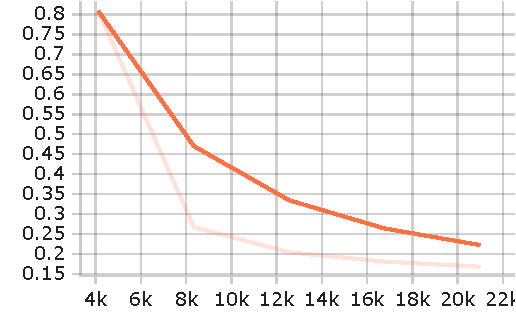
\includegraphics[width=\textwidth]{images/train_loss_epoch.pdf}
        \caption{Train Loss per Epoch}
        \label{fig:train_loss_epochs}
    \end{subfigure}
    \hfill
    \begin{subfigure}{0.48\textwidth}
        \centering
        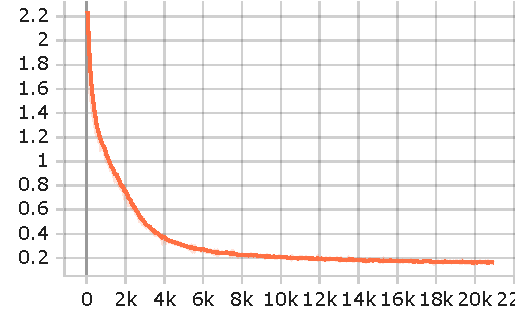
\includegraphics[width=\textwidth]{images/train_loss_step.pdf}
        \caption{Train Loss per Step}
        \label{fig:train_loss_steps}
    \end{subfigure}
\end{figure}

\subsection*{Question 2.8}

\subsubsection*{a)}

\textcolor{blue}{CODE}

\subsubsection*{b)}

To test the model on \textbf{Grimms' Fairy Tales} I used some prompts to test scenarios, characters and linguistic patterns:

\begin{itemize}
    \item \textbf{Prompt:} \textit{'Hansel said to'} \textbf{Temperature:} 0.8
    \item Model: Hansel said to Gretel: 'We shall soon find the way,' but they did not find it. They walked the whole night and all the next day too from morning till evening, but they did not get out of the forest
\end{itemize}

\begin{itemize}
    \item \textbf{Prompt:} \textit{'The wolf said to'} \textbf{Temperature:} 0.8
    \item Model: The wolf said to the Little Red-Cap, and then he said: 'See, Little Red-Cap, here is a piece
of cake and a bottle of wine; take them to your grandmother, she is ill
and weak, and they will do her finger.'
\end{itemize}

\begin{itemize}
    \item \textbf{Prompt:} \textit{'There was once'} \textbf{Temperature:} 0.8
    \item Model: There was once a man called Frederick: he had a wife whose name was
Catherine, and they had not long been married. One day Frederick said.
'Kate! I am going to work in the fields'
\end{itemize}

\begin{itemize}
    \item \textbf{Prompt:} \textit{'There was once'} \textbf{Temperature:} 0.8 \textbf{Do Sample:} True \textbf{Top-p:} 0.7
    \item Model: There was once upon a time a king who had a great forest near his
    palace, full of all kinds of wild animals. One day he sent out a
    huntsman to shoot him a roe, but he did not come back.
\end{itemize}

\begin{itemize}
    \item \textbf{Prompt:} \textit{'Rapunzel had'} \textbf{Temperature:} 1.0
    \item Model: Rapunzel had magnificent long hair, fine as spun gold, and when she
heard the voice of the enchantress she unfastened her braided tresses
\end{itemize}

\subsection*{Question 2.9}

\subsubsection*{a)}

\textcolor{blue}{CODE}

\subsubsection*{b)}

The benefits of Flash-Attention come from the nature of Load between Memory and Compute in the GPU. So basically, we have HBM (High Bandwidth Memory)
that is used to store, write and read the matrices $Q$, $K$ and $V$ and intermediate operations. HBM has a large memory, but is slow to compute things. Meanwhile, we have
SRAM (Static Random Access Memory) that is used to compute the intermediate results of the attention mechanism, since SRAM is fast to compute things.
In a normal attention mechanism:

\begin{itemize}
    \item The HBM loads the matrices $Q$ and $K$ into the SRAM
    \item SRAM computes the product $QK^T$ and writes it back to the HBM
    \item HBM loads the $QK^T$ into the SRAM
    \item SRAM computes the softmax and writes it back to the HBM
    \item HBM loads the $softmax(QK^T)$ and the $V$ matrix into the SRAM
    \item SRAM computes the final attention output and writes it back to the HBM
\end{itemize}

This process of loads and writes between the HBM and SRAM is slow and inefficient.
Flash Attention solves this problem by fusing all those operations into a single operation,
a so called fused-kernel, which is then loaded into the SRAM with the $Q$, $K$ and $V$ matrices. Then everything is computed in the SRAM
at once and written back to the HBM. This reduces the number of loads and writes between the HBM and SRAM, which makes the process
faster and more efficient.

This, in conjuction with the tilling techniques that break down large matrices into blocks that fit into the SRAM, are
what makes the Flash-Attention mechanism more efficient and faster than the normal attention mechanism. Indeed,
with flash-attention we can have a $O(n)$ complexity in memory, which is faster than the $O(n^2)$ complexity of the self-attention mechanism
and we have a speedup in the computation of the attention mechanism.

\newpage

\section*{Part 3}

\subsection*{Question 3.1}

\subsubsection*{a)}

For the first graph we have:

$[
[0, 1, 1, 0, 1],
[1, 0, 1, 0, 0],
[1, 1, 0, 1, 0],
[0, 0, 1, 0, 0],
[1, 0, 0, 0, 0]]$

For the second graph we have:

$[
[0, 1, 0, 0, 0, 0],
[1, 0, 1, 0, 1, 0],
[0, 1, 0, 1, 0, 0],
[0, 0, 1, 0, 1, 1],
[0, 1, 0, 1, 0, 1], 
[0, 0, 0, 1, 1, 0]]$

\subsubsection*{b)}

By squaring the first adjacency matrix we have:

$[
[3, 1, 1, 1, 0],
[1, 2, 1, 1, 1],
[1, 1, 3, 0, 1],
[1, 1, 0, 1, 0],
[0, 1, 1, 0, 1]]$

When we square the matrix $A \rightarrow A^2$, we are counting the number of paths of length 2 between each pair of nodes,
that is, $A_{ij}^2$ is the number of paths of length 2 between nodes $i$ and $j$.
For example the entry $A_{12}^2 = 1$ means that there is 1 path of length 2 between nodes 1 and 2, which is the path
$1 \rightarrow 3 \rightarrow 2$.

More generally, the entry $A_{uv}^n$ is the sum of the number of paths of length $n$ between nodes $u$ and $v$ in the graph.

\textbf{Note:} In the diagonals we have the number of paths of length 2 that start and end in the same node, for example,
if node $1$ and $5$ are connected this represents also a path of length 2, because we can go from node $1$ to node $5$ and
then back to node $1$ in this undirected graph.

\subsubsection*{c)}

The Laplacian matrix is defined as $L = D - A$, where $D$ is the degree matrix and $A$ is the adjacency matrix.
The degree matrix is a diagonal matrix where the diagonal entries are the degree of each node, that is, the number of edges
connected to each node.

For the second graph we have that $D$ is:

$[
[1, 0, 0, 0, 0, 0],
[0, 3, 0, 0, 0, 0],
[0, 0, 2, 0, 0, 0],
[0, 0, 0, 3, 0, 0],
[0, 0, 0, 0, 3, 0],
[0, 0, 0, 0, 0, 2]]$

And the Laplacian matrix is:

$[
[1, -1,  0, 0, 0, 0],
[-1, 3, -1, 0, -1, 0],
[0, -1,  2, -1, 0, 0],
[0, 0,  -1, 3, -1, -1],
[0, -1,  0, -1, 3, -1],
[0, 0,   0, -1, -1, 2]]$

By applying the Laplacian matrix to an input matrix $X$, we get $F = L \cdot X$. The resulting $F$ represents the transformed
feature values of the nodes. The Laplacian matrix $L$  can be seen as an operator on the rows of $X$, and the result
will depend on the structure of $L$, which 'encodes' the relationships between connected nodes.

The rows of $L$ correspond to the connections of each node to its neighbors. If a node has a higher degree, the corresponding row in 
$L$ will have more non-zero entries, meaning that the node's feature value will be influenced more by its neighbors.

Thus, the nodes that will change the most are those with the highest degree. In this case, nodes 2, 4, and 5,
each with degree 3, will experience the largest changes in feature values compared to nodes with lower degree.

\subsection*{Question 3.2}

\subsubsection*{a)}

The bias term defined as $B^{(l)}h_v^{(l)}$ allows to introduce a self-loop to each node in the graph, that is, it allows
a node $v$ to retain some of its previous information independent of the information from its neighbors. This is important,
since otherwise, the updated embedding $h_v^{(l+1)}$ would be completely dependent on the information from the neighbors
as seen in the term $\sum_{u \in N(v)} \frac{h_u^{(l)}}{|N(v)|}$, meaning it would dilute its unique characteristics.

\subsubsection*{b)}

Correlating with equation 6, we can see that that equation can be interpreted as simple instance of message passing, that is:

\begin{itemize}
    \item Message: The term $\frac{h_u^{(l)}}{|N(v)|}$ can be seen as the message passed from node $u$ to node $v$. Hence,
the $W^{(l)} \sum_{u \in N(v)} \frac{h_u^{(l)}}{|N(v)|}$ term can be seen as the aggregation of the messages from all neighbors of node $v$
where $W^{(l)}$ parametrizes how these messages are combined.
    \item Update: The term $B^{(l)}h_v^{(l)}$ and the activation function $\sigma$ can be seen as the update function that
incorporates the message from the neighbors and the node's own information to update the node's embedding.
\end{itemize}

\subsection*{Question 3.3}

\subsubsection*{a)}

Defining $D \in \mathbb{R}^{N \times N}$ as the degree matrix of the graph, we have that $D_{ii} = |N_v|$. We also define
$A \in \mathbb{R}^{N \times N}$ as the adjacency matrix of the graph with $A_{ij} = 1$ if there is an edge between nodes $i$ and $j$,
and $0$ otherwise. And define $H^{(l)} \in \mathbb{R}^{N \times D}$ as the matrix of node embeddings at layer $l$.

From equation 6, if we stack them for all nodes, we have that the update rule for all nodes can be written as:

\begin{align*}
    \begin{bmatrix}
        h_v^{(l+1)} \\
        \vdots \\
        h_N^{(l+1)}
    \end{bmatrix}
    & =  \begin{bmatrix}
        \sigma \left(W^{(l)} \sum_{u \in N(v)} \frac{h_u^{(l)}}{|N(v)|} + B^{(l)}h_v^{(l)}\right) \\
        \vdots \\
        \sigma \left(W^{(l)} \sum_{u \in N(v)} \frac{h_u^{(l)}}{|N(v)|} + B^{(l)}h_N^{(l)}\right)
    \end{bmatrix}  \\
\end{align*}

Now, instead of creating a higher dimensional tensor with a repeated weight matrix $W^{(l)}$ and a repeated bias matrix $B^{(l)}$,
we can rewrite with a single weight matrix $W^{(l)}$ and a single bias matrix $B^{(l)}$ by transposing it in the other side,
the same way we do it in batch dimensions in neural networks. We can then rewrite the equation as:

\begin{align*}
    H^{(l+1)} & = \sigma \left(  \left( \begin{bmatrix}
        \sum_{u \in N(1)} \frac{h_u^{(l)}}{|N(1)|} \\
        \vdots \\
        \sum_{u \in N(N)} \frac{h_u^{(l)}}{|N(N)|}
    \end{bmatrix} \right) W^{(l)^T} +  \begin{bmatrix}
        h_1^{(l)} \\
        \vdots \\
        h_N^{(l)}
    \end{bmatrix}
    B^{(l)^T}
    \right) \\
\end{align*}

Now, we can separate the terms $\frac{1}{|N(v)|}$ by using a matrix multiplication and knowing that, since $D$ is a diagonal matrix,
then its inverse is also a diagonal matrix with the inverse of the diagonal entries. We can then rewrite the equation as:

\begin{align*}
    H^{(l+1)} & = \sigma \left( \left(
        \begin{bmatrix}
            \frac{1}{|N(1)|} & 0 & \cdots & 0 \\
            0 & \frac{1}{|N(2)|} & \cdots & 0 \\
            \vdots & \vdots & \ddots & \vdots \\
            0 & 0 & \cdots & \frac{1}{|N(N)|}
        \end{bmatrix}
        \begin{bmatrix}
        \sum_{u \in N(1)} h_u^{(l)} \\
        \vdots \\
        \sum_{u \in N(N)} h_u^{(l)}
    \end{bmatrix} \right) W^{(l)^T} + \begin{bmatrix}
        h_1^{(l)} \\
        \vdots \\
        h_N^{(l)}
    \end{bmatrix} B^{(l)^T}
    \right) \\
    &=
    \sigma \left( \left(
        D^{-1}
        \begin{bmatrix}
            \sum_{u \in N(1)} h_u^{(l)} \\
            \vdots \\
            \sum_{u \in N(N)} h_u^{(l)}
        \end{bmatrix} \right) W^{(l)^T} + H^{(l)} B^{(l)^T}
    \right) \\
\end{align*}

Now, looking at the terms $\sum_{u \in N(v)} h_u^{(l)}$, we can see that we are summing the embeddings of the neighbors of node $v$.
Which is the same as summing over all nodes with a delta that is equal to one if there is an edge between nodes $v$ and $u$ and 0 otherwise. This
delta can be represented by the adjacency matrix $A$, meaning that that sum can be rewritten as $\sum_{v} A_{uv} h_u^{(l)}$.

Finally, we have that the update rule can be written as:

\begin{align*}
    H^{(l+1)} & = \sigma \left( \left(
        D^{-1}
        \begin{bmatrix}
        A_{11} & A_{12} & \cdots & A_{1N} \\
        A_{21} & A_{22} & \cdots & A_{2N} \\
        \vdots & \vdots & \ddots & \vdots \\
        A_{N1} & A_{N2} & \cdots & A_{NN}
    \end{bmatrix}
    \begin{bmatrix}
        h_1^{(l)} \\
        \vdots \\
        h_N^{(l)}
    \end{bmatrix}
    \right) W^{(l)^T} + \begin{bmatrix}
        h_1^{(l)} \\
        \vdots \\
        h_N^{(l)}
    \end{bmatrix} B^{(l)^T}
    \right) \\
    &=
    \sigma \left(
        D^{-1} A H^{(l)} W^{(l)^T}
     + H^{(l)} B^{(l)^T}
    \right) \\
\end{align*}

Hence, the final update rule for the graph convolutional network is:

\begin{align*}
    H^{(l+1)} & = \sigma \left(
        D^{-1} A H^{(l)} W^{(l)^T}
     + H^{(l)} B^{(l)^T}
    \right) \\
\end{align*}

Where $\sigma$ is applied row-wise.

Checking the dimensions, we have that $D^{-1} A H^{(l)} W^{(l)^T}$ is a product of a $N \times N$ matrix with a $N \times N$ with a $N \times D$ with a $D \times (D + 1)$,
which results in a $N \times (D + 1)$ matrix. The term $H^{(l)} B^{(l)^T}$ is a product of a $N \times D$ with a $D \times (D + 1)$, which results in a $N \times (D + 1)$ matrix.
Hence, the final output is a $N \times (D + 1)$ matrix, which is the same as the output matrix $H^{(l + 1)}$.

\subsubsection*{b)}

Median aggregation is a type of aggregation that is used to combine the information from the neighbors of a node in a graph
by taking the median of the embeddings of the neighbors. The problem is that Median aggregation is not a linear
operation, since it does not satisfy linear properties such as additivity and homogeneity. This means that the median
cannot be represented as a matrix multiplication, which is a linear operation.
Hence, the matrix form is not directly applicable to the median aggregation.

\subsection*{Question 3.4}

\subsubsection*{a)}

In GCNs, the weights used for aggregation are shared across all nodes. This means that the same set of weights is
used for aggregating the features of neighbors for each node in the graph. These weights are learned during
training, but remain uniform across nodes, that is, they do not vary depending on the node or its neighbors.

In GATs, the aggregation uses weights given by attention coefficients that are learned during training, which means that
the weights are different for each node and each neighbor. This allows the model to learn and assign different importance
to different neighbors. 

\subsubsection*{b)}

As explained in the previous question, the weights in GCNs are shared across all nodes meaning all neighbors contribute equally. This means the model is
less robust to noise since it cannot suppress the influence of some noisy neighbors. In GATs, the model can learn to assign
different importance to different neighbors, which allows it to suppress the influence of noisy neighbors and focus on the
most relevant ones. This makes GATs more robust to noise. With this being said, is expected that GCNs will have a lower
learned embedding quality than GATs.

\subsubsection*{c)}

A standard transformer applied to a sentence can be interpreted as a GNN if we consider the following structure: 

\begin{itemize}
    \item \textbf{Nodes:} Each token in the sentence is a node in the graph. The embeddings of the tokens are the node features.
    \item \textbf{Edges:} The edges in the graph are the connections between the tokens in the sentence, that is, the edges are defined by the attention mechanism.
The edge weights are the attention coefficients.
    \item \textbf{Graph Structure:} In a standard transformer, we are attending to all tokens in the sentence, which means that the graph is fully connected, that is,
each node is connected to every other node.
\end{itemize}

With this, we can make the following analogies:

\begin{itemize}
    \item The message passage in GNNs is equivalent to the attention mechanism in transformers, since the attention mechanism allows each token to attend to every other token in the sequence.
    \item The attention scores tell us the strength of the relationship between the tokens, which is similar to the edge weights in GNNs.
\end{itemize}

\subsubsection*{d)}

Two advantages of GATs over transformers are:

\begin{itemize}
    \item \textbf{Computational Efficiency}: Standard transformers compute the attention for all pairs of tokens in the sequence, meaning it has a global attention mechanism.
GATs compute attention only for the neighbors of each node, which makes them more computationally efficient and more scalable to larger graphs.
    \item \textbf{Interpretability and Graph Structure}: GATs are designed from the ground-up to work on graphs and capture the graph structure, where transformers require explicit encoding of the graph structure,
which is not intuitive for most problems. Besides that, GATs allow us to have a better interpretability of the model, since we can see the relationships between the nodes, while in transformers
we are not so much aware of this, since their attention mechanism is to focus on a token-level relationship, which might
not immediately translate to a graph structure/node relationship.
\end{itemize}






























\newpage
\bibliographystyle{abbrvnat}
\bibliography{references} 


\end{document}